\chapter{Implementierung}
\label{ch:implementation}
Die aufgestellten Anforderungen und das darauf basierende Design-Konzept kann nun in eine eigene Anwendung implementiert werden.
Dabei wird zuerst auf die Entwicklung auf iOS-Geräten eingegangen und anschließend die Technische Umsetzung dokumentiert.
Bei der Umsetzung wird auf die \Gls{i18n} geachtet, sodass es im Anschluss möglich ist die Anwendung mittels \Gls{l10n} in verschiedene Sprachen zu übersetzen.\pbreak%
%
Die Nutzung der Anwendung findet idealerweise auf einem Tablet statt, da dort mehr Platz für das Zeichnen und das Vornehmen von Einstellungen bereitsteht.
Für die Entwicklung wird die Entwicklungsumgebung \textit{Xcode} verwendet, welche Gerätesimulatoren für alle zur Verfügung stehenden iOS-Geräte bereitstellt.

\section{Entwicklung auf iOS-Geräten}
\label{sec:devios}
Wenn man einen nativen Ansatz verfolgt, um eine Anwendung auf iOS-Geräten zu entwickeln, stehen einem drei Technologien \textit{Objective-C}, \textit{Swift} und \textit{SwiftUI} zur Verfügung.
Außerdem wird die Entwicklungsumgebung Xcode, für dessen Nutzung ein macOS-Gerät notwendig ist, mit vielen hilfreichen Werkzeugen mitgeliefert.\pbreak%
%
Neben den Programmiersprachen selbst und den mitgelieferten Werkzeugen werden auch bestimmte Entwurfsmuster und Herangehensweisen empfohlen.
Die Kommunikation zwischen den bereitgestellten Schnittstellen des Herstellers und dem selbstentwickelten Programmcodes ist wesentlich einfacher und verständlicher, wenn man die selbe Architektur verwendet.
Es bleibt einem trotzdem selbst überlassen, wie man das eigene Projekt aufbauen möchte.
Im Falle dieser Thesis wird sich an den empfohlenen Herangehensweisen orientiert, die auch in den folgenden Abschnitten erklärt werden.

\subsection{Objective-C und Swift}
Objective-C war lange Zeit die einzige Programmiersprache für Geräte von Apple, bis Swift im Jahre 2014 angekündigt wurde.
Des Weiteren ist Swift Open-Source und verfolgt den Ansatz plattformübergreifend genutzt werden zu können \parencite{APP2020}.
Im Vergleich zu Objective-C hat Swift eine modernere Syntax und weniger Verbosität im Programmcode.
Es wird nicht mehr in Header- und Implementierungs-Dateien unterschieden und der gesamte Aufbau erinnert an eine Kombination verschiedenster moderner Programmiersprachen.
Dies lässt sich leicht erklären, da Chris \textcite{LAT} – Hauptentwickler der Programmiersprache Swift – auf seiner Website sagte \blockquote{Of course, it also greatly benefited from the experiences hard-won by many other languages in the field, drawing ideas from Objective-C, Rust, Haskell, Ruby, Python, C\#, CLU, and far too many others to list}.\pbreak%
%
Obwohl die Programmiersprachen Swift und Objective-C beide vom selben Hersteller sind und den selben Zweck erfüllen sollen, kann man die Unterschiede beider Sprachen sehr deutlich erkennen.
Im folgenden Listing \ref{lst:objc} wird eine Beispielimplementierung einer \texttt{Vehicle}-Klasse gezeigt. Diese Klasse beinhaltet eine Methode, die zum Öffnen eines Fensters gedacht ist.
Die Methode akzeptiert genau zwei Parameter, welche beide vom Datentyp \texttt{int} sein müssen.
Als ersten Parameter muss mit \texttt{percentage} der Prozentwert der Öffnung angegeben werden und als zweiten Parameter mit \texttt{seat} übergeben werden, welches Fenster geöffnet werden soll.
Im Anschluss wird ein Objekt der Klasse erstellt und die Methode aufgerufen.
\codelisting{Implementierung der Vehicle-Klasse in Objective-C}{lst:objc}{objc-example.m}{objc}
Anders als beim Objective-C Programmcode im Listing \ref{lst:objc} zu erkennen, entfällt bei einer Swift-Implementierung im Listing \ref{lst:swift} das Einbinden von Header-Dateien komplett.
Sowohl die Deklaration als auch die Definition der Methoden und Klassen erfolgt in nur einer Datei.
Des Weiteren erkennt man, dass Methodenaufrufe und Initialisierungen von Objekten um einiges klarer und leserlicher sind, da im Vergleich zu Objective-C die umschachtelnden eckigen Klammern (\texttt{[} und \texttt{]}) entfallen.
\codelisting{Implementierung der Vehicle-Klasse in Swift}{lst:swift}{swift-example.swift}{swift}

\subsection{SwiftUI}
Seit 2019 gibt es auch die Möglichkeit mittels \textit{SwiftUI} mobile Anwendungen für Apple Geräte zu entwickeln.
SwiftUI ist dabei weniger eine eigene Sprache, sondern eher ein deklarativer Ansatz in Swift Benutzeroberflächen zu bauen.
In einfachen Swift Projekten mit dem Ziel eine iOS-Anwendung zu entwickeln wird für die Benutzeroberfläche das Framework \textit{UIKit} verwendet.
SwiftUI soll in Zukunft UIKit ablösen, sodass alle Anwendungen in Zukunft mittels SwiftUI entwicklet werden können.\pbreak%
%
Da SwiftUI noch relativ jung ist und regelmäßig neue Funktionen implementiert werden ist es für eine komplexere Anwendung ungeeignet.
Einfache Notizen- oder Todo-Apps lassen sich schnell und einfach bauen, doch für das Zeichnen auf Kartendaten müsste wieder auf das Framework UIKit zurückgegriffen werden.
Das hat damit zu tun, dass viele Komponenten noch nicht kompatibel für SwiftUI gemacht wurde und im Hintergrund weiterhin auf UIKit basieren.
Unter diesem Komponenten befindet sich auch die \texttt{MKMapView} aus dem \texttt{MapKit} Framework, die für das Darstellen einer Karte benötigt wird.
Es wäre theoretisch möglich die Map View innerhalb einer SwiftUI-Ansicht anzuzeigen, allerdings müsste auch hier für ein tieferes Eingreifen in die Funktionen der Map View wieder auf Swift mit UIKit zurückgegriffen werden.
Aus diesem Grund ist es sinnvoller, für die zu entwickelnde Anwendung, auf SwiftUI zu verzichten.

\subsection{Entwurfsmuster}
Es gibt viele verschiedene Möglichkeiten die Architektur einer Software aufzubauen.
Bei einfachen iOS-Anwendungen wird dafür das Entwurfsmuster \ac{mvc} verwendet.
Obwohl es möglich ist für die eigene Anwendung ein anderes Entwurfsmuster zu verwenden, lohnt es sich das bereitgestellte zu nutzen, da das \Gls{sdk} viele Werkzeuge mitbringt, die automatisiert Dateien erstellen und verwalten können, solange man sich an das \ac{mvc}-Entwurfsmuster hält.
\subsubsection{Model-View-Controller}
Das \ac{mvc}-Entwurfsmuster teilt den Programmcode in die drei Bereiche \textit{Model}, \textit{View} und \textit{Controller} auf.
Jeder dieser Bereiche hat eine eigene Zuständigkeit und sollte bis auf die Kommunikation streng von den anderen getrennt sein.
Die Einteilung ermöglicht eine bessere Wartbarkeit und Wiederverwendbarkeit von Programmcode.\\[10pt]
\begin{figure}[h!]
	\centering
	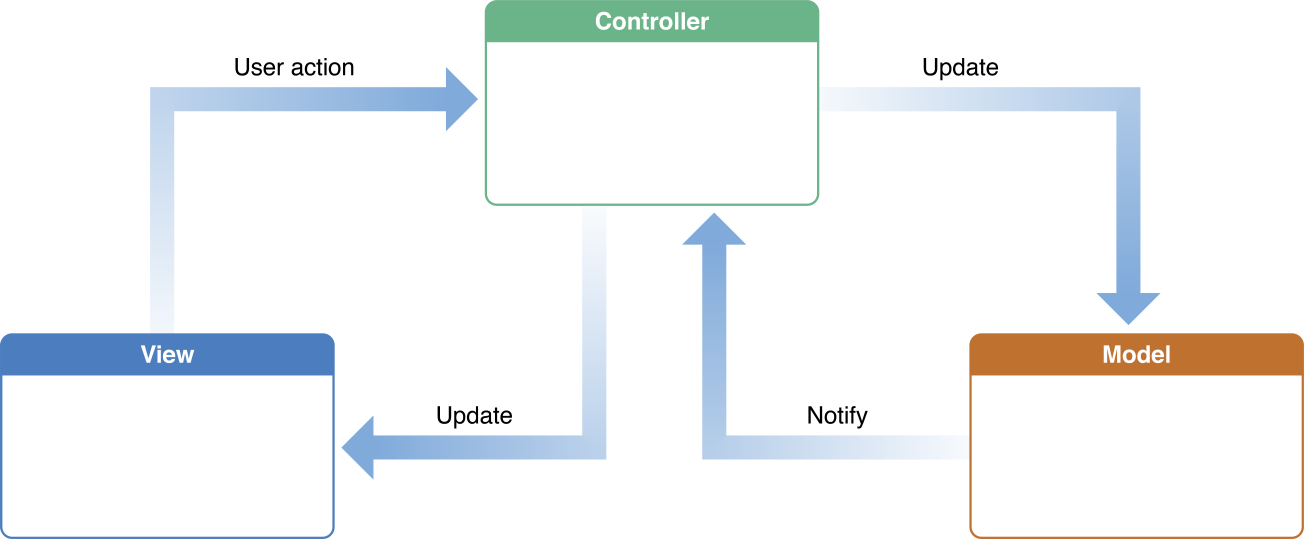
\includegraphics[scale=0.3]{images/model-view-controller}
	\caption{Darstellung der Model-View-Controller Beziehungen \parencite{APP2018}}
	\label{fig:model-view-controller}
\end{figure}
\pbreak%
Der \textbf{Model}-Bereich beinhaltet in erster Linie den Code für das Datenmodell der Anwendung, allerdings können aber auch Hilfsklassen enthalten sein, die oft verwendeten Code zusammenfassen.
Ein Model sollte nie selbst eine Referenz zu einer View oder einem Controller haben, sondern ein Controller oder eine View den Verweis zum Model.
Wie man der Abbildung \ref{fig:model-view-controller} entnehmen kann wartet das Model darauf, dass es eine Aufgabe vom Controller erhält und informiert diesen gegebenenfalls sobald die Aufgabe erfüllt wurde.\pbreak%
%
Die \textbf{View} ist der Bereich, mit dem der Benutzer interagiert.
Programmcode im View-Bereich sollte keine Geschäftslogik enthalten, sondern nur Code, welcher die View aktualisiert.
Dies könnte zum Beispiel Programmlogik zum bedingten Einfärben eines Buttons sein.
Wenn eine View Geschäftslogik benötigt, um bestimmte Aufgaben zu erfüllen, dann wird ein Verweis zu einem Model erzeugt, in dem die Geschäftslogik enthalten ist.
Auch in diesem Fall wartet die View auf Aufgaben eines Controller, welcher zum Beispiel ein Aktualisieren der Ansicht anfordert.
Andersherum kann die View den Controller darüber informieren, dass der Benutzer eine Aktion getätigt hat, wie zum Beispiel das Drücken eines Buttons.\pbreak%
%
Die Aufgabe der \textbf{Controller} ist es zwischen den Views und den Models zu vermitteln.
Wenn es zum Beispiel Änderungen ein einem Model gibt, dessen Daten direkt an eine Ansicht gebunden sind, muss der Controller der entsprechenden View Bescheid geben die Ansicht zu aktualisieren.
Ebenso muss der Controller das Model aktualisieren, wenn der Benutzer eine Aktion auf der Benutzeroberfläche geändert hat, welche direkt mit dem Model verbunden ist.
Wie Kommunikation zwischen den drei Komponenten funktioniert kann bei jeder Implementierung des \ac{mvc}-Entwurfsmuster unterschiedlich sein.
Bei einem iOS-Projekt wird standardmäßig das \textit{Delegation-Pattern} verwendet.

\subsubsection{Delegation-Pattern}
Das Delegation-Pattern erlaubt es bestimmte Logik über ein anderes Objekt abzubilden – also die Aufgabe zu delegieren.
Dabei kann man ein anderes Objekt einfach benachrichtigen, dass es nun etwas tun soll oder das andere Objekt etwas ``fragen`` und mit der Antwort weiterarbeiten.
In der Entwicklung von iOS-Geräten ist das Delegation-Pattern tief verwurzelt, da es in den Schnittstellen der meisten Funktionen eingebaut ist.
Möchte man innerhalb einer Anwendung auf die Ortungsdaten zugreifen, kommt man um das Delegation-Pattern nicht herum.\pbreak%
%
Um auf die Ortungsdaten zugreifen zu können würde man aus dem Framework \texttt{CoreLocation} die Klasse \texttt{CLLocationManager} nutzen.
Diesem Location Manager müsste man eine Referenz zur eigenen Klasse – beziehungsweise eine Referenz zu der Klasse, in welcher die Daten als Antowort ankommen sollen – mitgeben, die das entsprechende \Gls{protocol}, in diesem Fall \texttt{CLLocationManagerDelegate}, implementiert.
Sobald der Location Manager die Ortungsdaten des Benutzers erfasst hat nutzt er die zuvor mitgegebene Referenz zur entsprechenden Klasse und ruft dort die Funktion \texttt{locationManager(manager:didUpdateLocations:)} auf, in der die Ortungsdaten übermittelt werden.
Diese Funktion muss existieren, da dem genannten \Gls{protocol} zugestimmt wurde und es deshalb implementiert werden muss.
Fehlt die Implementierung der Funktion in der Referenz, handelt es sich dabei um einen Syntax-Fehler und das Programm kann nicht kompiliert werden.\pbreak%
%
Um die Funktionsweise des Delegation-Patterns besser darstellen zu können, wird im Folgenden Beispiel der Programmcode bei einer Delegation erläutert.
Im Listing \ref{lst:engine} wird die \texttt{Vehicle}-Klasse dahingehend erweitert, dass man mit der Methode \texttt{turnKey()} den Motor starten kann (Zeile 4).
In der \texttt{Engine}-Klasse brauchen wir eine Referenz zum Fahrzeug, da der verbrauchte Kraftstoff des Fahrzeugs in der \texttt{run()}-Methode abgezogen werden muss (Zeile 17 bis 22).
Das jetzt entstandene Problem ist, dass es eine direkte Beziehung zwischen Fahrzeug und Motor gibt und die \texttt{Engine}-Klasse nicht abstrakt eingesetzt werden kann.\\
\codelisting{Implementierung der Engine-Klasse ohne Delegation}{lst:engine}{engine.swift}{swift}

Bestimmte Aufgabenbereiche kann der Motor daher an die \texttt{Vehicle}-Klasse delegieren.
Dabei muss der Motor gar nicht wissen, ob es sich dabei wirklich um die \texttt{Vehicle}-Klasse handelt oder eine andere beliebige Klasse.
Es wird als Motor nur weitergegeben, dass soeben ein Liter Kraftstoff verbraucht wurde und der Delegierte soll mit dieser Information weiterarbeiten.
Die einzige Bedingung, die von der Referenz erfüllt werden muss, ist das Implementieren des entsprechenden \Glspl{protocol}.
Dabei ist es egal welche Klasse das \Gls{protocol} implementiert.
\codelisting{Implementierung der Engine-Klasse mit Delegation}{lst:engine-del}{engine-delegation.swift}{swift}

In den Zeilen 1 bis 4 des Listings \ref{lst:engine-del} wird ein \Gls{protocol} erstellt.
Die \texttt{Vehicle}-Klasse, welches diesem \Gls{protocol} in Zeile 6 zustimmt muss die dort definierten Funktionen implementieren.
In der Zeile 10 wird dem Motor nicht mehr die Referenz zum Fahrzeug selbst übergeben, sondern zu einer beliebigen Klasse, die das \texttt{EngineDelegate}-\Gls{protocol} implementiert.
Der Motor kann absofort in den Zeilen 30 bis 35 die implementierten Funktionen aufrufen, da die Klasse sich sicher sein kann, dass die Referenz das \texttt{EngineDelegate}-\Gls{protocol} implementiert.
Im iOS-Umfeld verteilen die Controller auf diese Weise Daten zwischen den verschiedenen Ansichten.

\subsection{View Controller Lifecycle}
Für die Anzeige von Inhalten werden \textit{View Controller} verwendet.
In einer \textit{Getting Started}-Anleitung beschreibt \textcite{APP2016} den Aufbau und die Funktionsweise eines solchen Controllers, welche an dieser Stelle wiedergegeben wird.
Diese Controller bieten Grundfunktionalitäten, um Views auf dem Bildschirm anzuzeigen.
Dabei werden im Hintergrund von dem System bestimmte Funktionen aufgerufen, die sich überschreiben lassen, sodass eigene Logik hinzugefügt werden kann.
Welche Funktionen wann aufgerufen werden wird als der \textit{View Controller Lifecycle} bezeichnet.
\begin{figure}[h!]
	\centering
	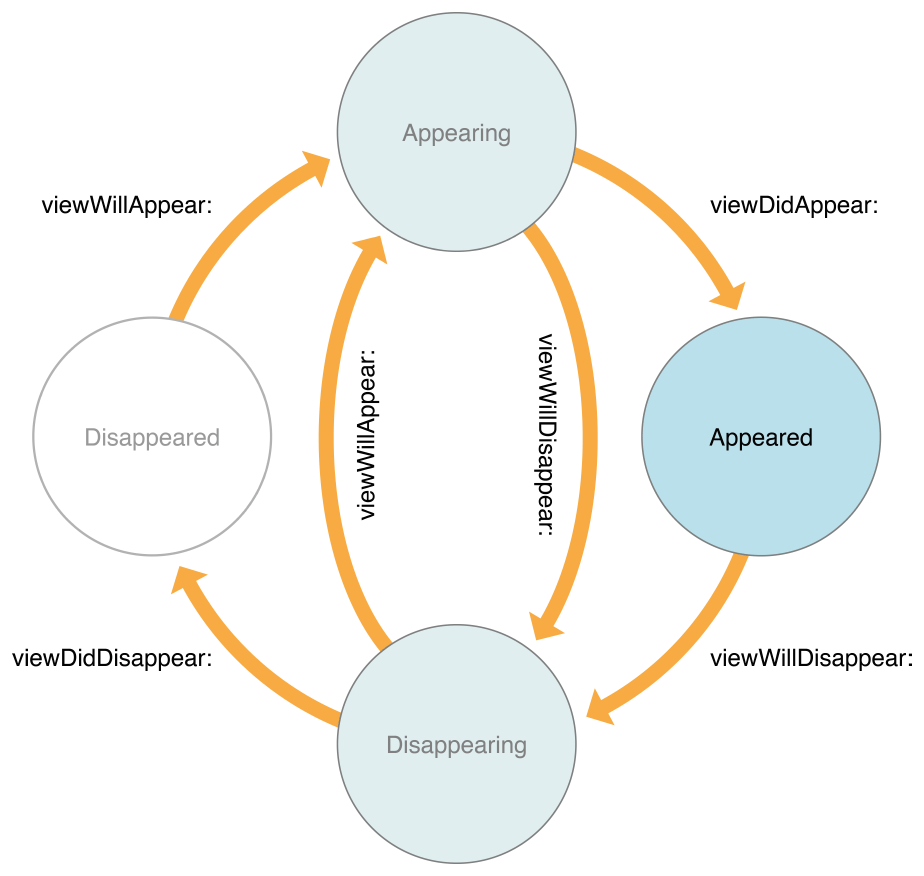
\includegraphics[scale=0.5]{images/view-controller-lifecycle}
	\caption{Darstellung des View Controller Lifecycles \parencite{APP2016}}
	\label{fig:view-controller-lifecycle}
\end{figure}
\begin{description}
\item[\texttt{viewDidLoad()}]
Wird nur einmal in einer View Controller Instanz aufgerufen.
An dieser Stelle wurde der View Controller bereits initialisiert und im Speicher abgelegt.
Benutzerdefinierter Initialisierungscode kann hier eigene Views erstellen oder Referenzen zu Models herstellen.
\item[\texttt{viewWillAppear()}]
Wird jedesmal aufgerufen, bevor die Content View des View Controllers, welche alle visuellen Komponenten enthält, angezeigt wird.
Bei Animationen zwischen den Ansichten wird diese Methode vor der Animation aufgerufen.
\item[\texttt{viewDidAppear()}]
Wird jedesmal aufgerufen, nachdem die Content View des View Controllers angezeigt wurde.
Falls eine Animation zum Anzeigen verwendet wird, kann an dieser Stelle darauf reagiert werden, wenn die Animation abgeschlossen ist.
Wichtig zu beachten ist dabei, dass die Content View nicht unbedingt sichtbar sein muss.
Es kann vorkommen, dass der Inhalt sich hinter einer anderen Ansicht befindet.
\item[\texttt{viewWillDisappear()}]
Analog zu \texttt{viewWillAppear()} wird diese Methode jedesmal aufgerufen, wenn die Content View des View Controllers von der Ansicht entfernt werden soll.
Auch hier können vorbereitende Aufgaben durchgeführt werden, wie eine Animation anzustoßen.
\item[\texttt{viewDidDisappear()}]
Analog zu \texttt{viewDidAppear()} wird diese Methode jedesmal aufgerufen, wenn die Content View des View Controllers von der Ansicht entfernt wurde.
\end{description}
Bei Aufruf der Methoden \texttt{viewWillAppear()} und \texttt{viewDidDisappear()} ist die Content View im jeden Fall nicht sichtbar, sodass es sich an diesen Stellen eignet die Benutzeroberfläche zu aktualisieren.
Findet eine Aktualisierung der Benutzeroberfläche von zum Beispiel Texten oder Listenpunkten statt, während die Content View sichtbar ist, kann der Benutzer die abrupte Änderung sehen.\pbreak%
%
Alle vorgestellten Methoden haben eine Standardimplementierung und müssen nicht überschrieben werden.
Falls eine dieser Methoden überschrieben wird, sollte die Standardimplementierung trotzdem hinzugezogen werden.
Aus diesem Grund sollte in jedem Fall am Anfang der eigenen Implementierung die Implementierung der Oberklasse ausgeführt werden.
Dies kann in der Programmiersprache Swift mit dem \texttt{super}-Keyword erreicht werden, wie im Listing \ref{lst:override} zu sehen ist.\\
\codelisting{Überschreiben einer View Controller Lifecycle Methode}{lst:override}{override.swift}{swift}

\subsection{Die Information Property List}
In jedem iOS-Projekt muss eine sogenannte \textit{Information Property List} vorhanden sein.
Diese kann als \texttt{Info.plist}-Datei an einer beliebigen Stelle im Projekt abgelegt sein, es muss nur der Pfad zu ihr hinterlegt werden.
Die Property List ist ein Key-Value-Store und basiert auf XML (siehe Listing \ref{lst:plist}).
In dieser Liste werden unter anderem der Name der Anwendung, die Version und die Buildnummer hinterlegt, sowie weitere Einstellungen vorgenommen.
Außerdem werden in der Property List auch die Begründungstexte für Berechtigungsanfragen abgelegt.
Wenn eine Anwendung versucht den Zugriff auf das Mikrofon anzufragen, allerdings kein Begründungstext hinterlegt wurde, der dem Benutzer angezeigt werden kann, wird die Berechtigung nicht angefragt.
\codelisting{Beispielinhalt einer Property List}{lst:plist}{plist-example.plist}{xml}\\
In der Information Property List können auch eigene Werte hinterlegt werden, die sowohl in der Anwendung selbst abgefragt werdne können als auch in den Buildprozessen der Anwendung verwendet werden können.

\section{Technische Umsetzung}
\label{sec:techimp}
\subsection{Autolayout}
\subsection{JSON Encoding und Decoding}
\subsection{Generics}
\subsection{Gesture Recognizers}
\subsection{MapKit Overlays}

\section{Lokalisierung der Anwendung}
\label{sec:localizing}
\subsection{Localizable-Dictionary}
\subsection{ISO Country Codes}
